\section{Builtins} \label{sec:builtins}

From a prover's perspective, the difficulty of different function modules in a ZKVM varies, hence, we are utilizing a modular architecture, decoupling the different modules to the maximum extent possible. When dealing with complex modules, the circuit scale vastly grows in size increasing the cost of the proof, in addition to potentially not being frequently used, creating inefficiencies. We utilize builtins to enhance this. Through Plookup technology we are able to store the circuit overhead upon usage, enabling us to flexibly handling the overhead problem of complex circuits.

\subsection{Range Check}

In order to implement Range Check we are utilizing Lookup Argument technology. Please refer to Section \ref{sec:key-technologies} for detailed design. The basic fixed table is an 8-bit lookup table, i.e.\ 0-255. For 8-bit numbers, the validity is checked using Plookup. The utilization of Plookup check is shown in Figure \ref{fig:rangecheck-lookup}.
\begin{figure}[!ht]
    \centering
    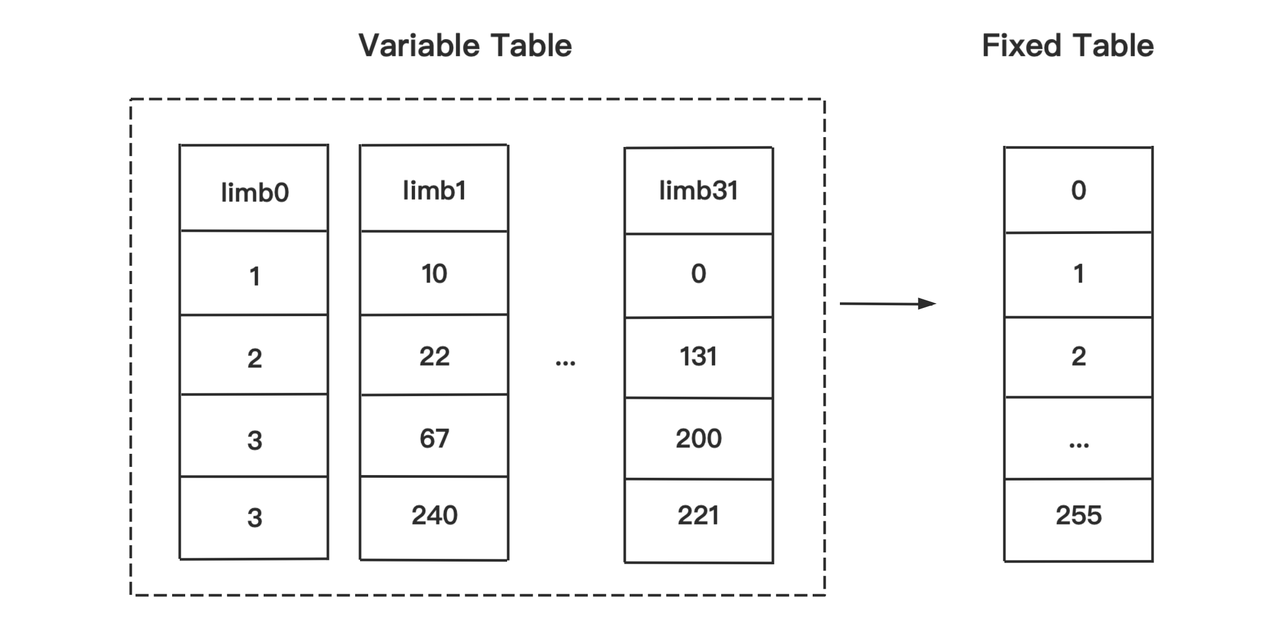
\includegraphics[width=0.8\textwidth]{rangecheck-lookup.png}
    \caption{Fixed/Variable lookup table}
    \label{fig:rangecheck-lookup}
\end{figure}

For numbers greater than 8 bits, break them down to multiple 8-bit limbs and perform Plookup respectively, and then check the constraints of sum and limbs. Take 256-bit as an example,
$\text{integer256} = \text{limb}_0 + \text{limb}_1 \cdot 2^8 + \text{limb}_2 \cdot (2^8)^2 + \text{limb}_3 \cdot (2^8)^3 + \cdots + \text{limb}_{31} \cdot (2^8)^{31}$.

\subsection{Bitwise}

Lookup Arguments are also utilized to implement most of the bitwise operations. The basic lookup table is based on 8 bits, containing three columns, two inputs and one bitwise output, as shown in Table \ref{table:bitwise-lookup}.

\begin{table}[!ht]
    \centering
    \begin{tabular}{|l|l|l|l|}
    \hline
        & \emph{lhs} & \emph{rhs} & \emph{out} \\ \hline
        BitwiseAND table & lhs = 8-bit & rhs = 8-bit & lhs AND rhs \\ \hline
        BitwiseOR table & lhs = 8-bit & rhs = 8-bit & lhs OR rhs \\ \hline
        BitwiseXOR table & lhs = 8-bit & rhs = 8-bit & lhs XOR rhs \\ \hline
    \end{tabular}
    \caption{Bitwise lookup table}
    \label{table:bitwise-lookup}
\end{table}

Bitwise operations larger than 8 bits are broken down into multiple 8-bit operations with Plookup ran on each operation. Take the 32-bit AND of two numbers as an example,
\begin{align*}
a \land b &= (a_0 + a_1\cdot2^8 + a_2 \cdot (2^8)^2 + a_3\cdot(2^8)^3) \land (b_0 + b_1\cdot2^8 + b_2 \cdot (2^8)^2 + b_3\cdot(2^8)^3)\\ &= (a_0 \land b_0) + (a_1 \land b_1)\cdot2^8 + (a_2 \land b_2)\cdot(2^8)^2+(a_3 \land b_3)\cdot(2^8)^3.
\end{align*}

Therefore, for two $n$-bit numbers $a$ and $b$, let $m=n/8$, and $a_i,b_i$ are their limbs, then
\begin{align*}
a \land b &= \sum_{i=0}^{m-1} (2^{8i} \cdot (a_i \land b_i)), \\
a \lor b &= \sum_{i=0}^{m-1} (2^{8i} \cdot (a_i \lor b_i)), \\
a \oplus b &= \sum_{i=0}^{m-1} (2^{8i} \cdot (a_i \oplus b_i)).
\end{align*}

The implementation of NOT is slightly different. The NOT to constrain $a$ is
\[ \neg a + a = 2^{256} - 1. \]

\subsection{Sinsemilla Hash}

We use Halo2 \cite{website:halo2} Sinsemilla Hash scheme.

For detailed design of the hash algorithm and the parameters used below, please refer to Section \ref{sec:key-technologies}.
Following is the main calculation process of Sinsemilla:
\begin{enumerate}
    \item Set the initial value $\mathrm{Acc}_0 = Q$
    \item Perform loop calculation of $i$ from $0$ to $n-1$:
    \[ \mathrm{Acc}_{i+1} = (\mathrm{Acc}_i + P_{m_{i+1}}) + \mathrm{Acc}_i. \]
\end{enumerate}

Now, let $R_i = \mathrm{Acc}_i + P_{m_{i+1}}$, then $\mathrm{Acc}_{i+1} = R_i + \mathrm{Acc}_i$ then according to previous definition, we have
\begin{align*}
\lambda_{1,i} &= \frac {y_{Acc,i} - y_{P,i}}{x_{Acc,i}-x_{P,i}}, \\
x_{R,i} &= \lambda_{1,i}^2 - x_{\text{Acc},i}-x_{P,i}, \\
y_{R,i} &= \lambda_{1,i} (x_{\text{Acc},i} - x_{R,i}) - y_{\text{Acc},i}, \\
\lambda_{2,i} &= \frac {y_{\text{Acc},i} - y_{R,i}}{x_{\text{Acc},i}-x_{R,i}}, \\
x_{\text{Acc},i+1} &= \lambda_{2,i}^2 - x_{\text{Acc},i}-x_{R,i}, \\
y_{\text{Acc},i+1} &= \lambda_{2,i} (x_{\text{Acc},i} - x_{\text{Acc},i+1}) - y_{\text{Acc},i}.
\end{align*}

So, we have constrains as in Table \ref{table:raw-sinsemilla-hash-constraints}.
\begin{table}[!ht]
    \centering
    \begin{tabular}{|c|l|l|}
    \hline
    \emph{Degree} & \emph{Constraints} & \emph{Notes} \\
    \hline
    3 & $q_\text{incomplete-add} \cdot (x_{R,i} + x_{\text{Acc},i} + x_{P,i} - \lambda_{1,i}^2) = 0$
    & $x_{R,i} = \lambda_{1,i}^2 - x_{\text{Acc},i} - x_{P,i}$ \\
    3 & $q_\text{incomplete-add} \cdot (\lambda_{1,i} (x_{\text{Acc},i} - x_{R,i}) - (y_{\text{Acc},i} + y_{R,i})) = 0$
    & $y_{R,i} = \lambda_{1,i} (x_{\text{Acc},i} - x_{R,i}) - y_{\text{Acc},i}$ \\
    3 & $q_\text{incomplete-add} \cdot (\lambda_{1,i} (x_{\text{Acc},i} - x_{P,i}) - (y_{\text{Acc},i} - y_{P,i})) = 0$
    & $\lambda_{1,i} = (y_{\text{Acc},i} - y_{P,i}) / (x_{\text{Acc},i}-x_{P,i})$ \\
    3 & $q_\text{incomplete-add} \cdot (x_{\text{Acc},i+1} + x_{\text{Acc},i} + x_{R,i} - \lambda_{2,i}^2) = 0$
    & $x_{\text{Acc},i+1} = \lambda_{2,i}^2 - x_{\text{Acc},i}-x_{R,i}$ \\
    3 & $q_\text{incomplete-add} \cdot (\lambda_{2,i} (x_{\text{Acc},i} - x_{\text{Acc},i+1}) - (y_{\text{Acc},i} + y_{\text{Acc},i+1})) = 0$
    & $y_{\text{Acc},i+1} = \lambda_{2,i} (x_{\text{Acc}_,i} - x_{\text{Acc},i+1}) - y_{\text{Acc},i}$ \\
    3 & $q_\text{incomplete-add} \cdot (\lambda_{2,i} (x_{\text{Acc},i} - x_{R,i}) - (y_{\text{Acc},i} - y_{R,i}) ) = 0$
    & $\lambda_{2,i} = (y_{\text{Acc},i} - y_{R,i}) / (x_{\text{Acc}_i}-x_{R,i})$ \\
    \hline
    \end{tabular}
    \caption{Sinsemilla Hash constraints}
    \label{table:raw-sinsemilla-hash-constraints}
\end{table}
\begin{align*}
    & \lambda_{2,i} = \frac {y_{\text{Acc},i} - y_{R,i}}{x_{\text{Acc},i}-x_{R,i}} \\
    \implies & y_{\text{Acc},i} - y_{R,i} = \lambda_{2,i} (x_{\text{Acc},i}-x_{R,i}), \\
    & y_{R,i} = \lambda_{1,i} (x_{\text{Acc},i} - x_{R,i}) - y_{\text{Acc},i} \\
    \implies & y_{\text{Acc},i} - (\lambda_{1,i} (x_{\text{Acc},i} - x_{R,i}) - y_{\text{Acc},i}) = \lambda_{2,i} (x_{\text{Acc},i}-x_{R,i}) \\
    \implies & 2y_{\text{Acc},i} = (\lambda_{1,i} + \lambda_{2,i}) (x_{\text{Acc},i}-x_{R,i}).
\end{align*}

Therefore, the check for $\lambda_{2,i} = (y_{\text{Acc}_i} - y_{R,i})/(x_{\text{Acc}_i}-x_{R,i})$ can be replaced by
\[ q_\text{incomplete-add} \cdot (\lambda_{2,i} (x_{\text{Acc},i} - x_{R,i}) - (y_{\text{Acc},i} - y_{R,i}) ) = 0, \]

then
\[ q_\text{incomplete-add} \cdot ((\lambda_{2,i} + \lambda_{1,i}) (x_{\text{Acc},i} - x_{R,i}) - 2y_{\text{Acc},i}) = 0. \]

We haven't used $y_{R,i}$ of $R_i = \{x_{R,i}, y_{R,i}\}$ in the second step of checking for $\mathrm{Acc}_{i+1} = R_i + \mathrm{Acc}_i$. Therefore, remove the constraint on $y_{R,i}$ in the first step and the entire constraint develop into what is displayed in Table \ref{table:simplified-sinsemilla-hash-constraints}.

\begin{table}[!ht]
    \centering
    \begin{tabular}{|c|l|l|}
        \hline
        \emph{Degree} & \emph{Constraints} & \emph{Notes} \\
        \hline
        3 & $q_\text{incomplete-add} \cdot (x_{R,i} + x_{\text{Acc},i} + x_{P,i} - \lambda_{1,i}^2) = 0$
        & $x_{R,i} = \lambda_{1,i}^2 - x_{\text{Acc},i} - x_{P,i}$ \\
        3 & $q_\text{incomplete-add} \cdot (\lambda_{1,i} (x_{\text{Acc},i} - x_{P,i}) - (y_{\text{Acc},i} - y_{P,i})) = 0$
        & $\lambda_{1,i} = (y_{\text{Acc},i} - y_{P,i}) / (x_{\text{Acc},i}-x_{P,i})$ \\
        3 & $q_\text{incomplete-add} \cdot (x_{\text{Acc},i+1} + x_{\text{Acc},i} + x_{R,i} - \lambda_{2,i}^2) = 0$
        & $x_{\text{Acc},i+1} = \lambda_{2,i}^2 - x_{\text{Acc},i}-x_{R,i}$ \\
        3 & $q_\text{incomplete-add} \cdot (\lambda_{2,i} (x_{\text{Acc},i} - x_{\text{Acc},i+1}) - (y_{\text{Acc},i} + y_{\text{Acc},i+1})) = 0$
        & $y_{\text{Acc},i+1} = \lambda_{2,i} (x_{\text{Acc},i} - x_{\text{Acc},i+1}) - y_{\text{Acc},i}$ \\
        3 & $q_\text{incomplete-add} \cdot ((\lambda_{2,i} + \lambda_{1,i}(x_{\text{Acc},i} - x_{R,i}) - 2y_{\text{Acc},i} ) = 0$
        & $\lambda_{2,i} = (y_{\text{Acc},i} - y_{R,i}) / (x_{\text{Acc},i}-x_{R,i})$ \\
        \hline
    \end{tabular}
    \caption{Simplified Sinsemilla Hash constraints}
    \label{table:simplified-sinsemilla-hash-constraints}
\end{table}

\subsection{Comparison}

Range Check is used to perform \verb|GTE| comparison, using Cairo's scheme \cite{cryptoeprint:2021/1063}.

On a circuit level, we only need to support 3 comparisons: \verb|EQ|, \verb|GTE| and \verb|NEQ|. We will perform 256-bit Range Check for two numbers to be compared, and then perform a 256-bit Range Check for the difference between two numbers.

\verb|EQ| checks the equality of two 256-bit numbers $a$ and $b$. The constraint is $a-b=0$.

\verb|NEQ| checks the inequality of two 256-bit numbers $a$ and $b$. The constraint is $(a-b)\cdot(a-b)^{-1}=1$.

\verb|GTE| checks whether two 256-bit numbers $a$ and $b$ satisfy $a \geq b$.

First, use Range Check to constrain each number in 256 bits, and then compare them according to the difference. If the difference exceeds 256 bits, it means that they don't satisfy $a \geq b$. The constraint pseudo code is
\begin{lstlisting}[language=Rust]
range_check(integer256_a, range256bit)
range_check(integer256_b, range256bit)
let diff = integer256_a - integer256_b
range_check(diff, range256bit)
\end{lstlisting}

We can combine \verb|GTE| and \verb|NEQ| with bitwise operations to perform other comparisons, listed in Table \ref{table:comparison-level}.
\begin{table}[!ht]
    \centering
    \begin{tabular}{|l|l|}
    \hline
        \emph{Application level} & \emph{Circuit level} \\ \hline
        $a \ge b$ & a \verb|GTE| b \\
        $a \le b$ & b \verb|GTE| a \\
        $a > b$ & (a \verb|GTE| b) \&\& (a \verb|NEQ| b) \\
        $a < b$ & (b \verb|GTE| a) \&\& (b \verb|NEQ| a) \\ \hline
    \end{tabular}
    \caption{Comparison level}
    \label{table:comparison-level}
\end{table}

\subsection{Signature}

We support two different signature schemes, ECDSA \cite{Johnson99theelliptic} and Schnorr \cite{jofc-1991-14302}.

\subsubsection{ECDSA Signature}

The hash function we choose is Sinsemilla Hash, which is the same function used in signature generation. With the following notations:
\begin{itemize}
    \item $(r, s)$ is the signature.
    \item $m$ is the message to verify.
    \item $Q(Q_x, Q_y)$ is the public-key curve point.
    \item $h$ is the hash result of $m$.
    \item $G$ is the elliptic curve base point.
    \item $n$ is the order of $G$.
    \item $\mathcal{O}$ is the identity element.
    \item $L_n$ is the bit length of $n$.
\end{itemize}

The constraints are the following:
\begin{enumerate}
    \item Check that $Q$ is not equal to $\mathcal{O}$.
    \item Check that $Q$ lies on the curve, which means: $Q_y^2 = Q_x^3+\alpha Q_x + \beta$.
    \item Check that $nQ = \mathcal{O}$.
    \item Check that $r$ and $s$ are in $[1, n-1]$.
    \item Let $z$ be the leftmost $L_n$ bits of $h$ (we use Sinsemilla Hash builtin circuit to check $h \equiv \mathrm{HASH}(m)$).
    \item Calculate $u_1 = zs^{-1} \bmod n$ and $u_2 = rs^{-1} \bmod n$.
    \item Calculate curve point $(x_1,y_1) = u_1 G + u_2 Q$, check $(x_1, y_1) \ne \mathcal{O}$.
    \item Check that $r \equiv x_1 \pmod n$.
\end{enumerate}

\subsubsection{Schnorr Signature}

Schnorr signature is known for its simplicity, Bitcoin used Schnorr signature as well. The hash function we choose is Sinsemilla Hash. With the following notations:
\begin{itemize}
    \item $(s, e)$ is the signature.
    \item $m$ is the message to verify, it is represented as list of finite bit strings.
    \item $h$ is the hash result of $m$.
    \item $g$ is the generator.
    \item $y$ is the public verification key.
\end{itemize}

The constraints are the following:
\begin{enumerate}
    \item Check $r_v = g^s y^e$.
    \item Check $e_v = \mathrm{Hash}(r_v \mathbin{||} m)$, where $||$ denotes concatenation, $r_v$ is represented as a bit string (Like above, we use Sinsemilla Hash builtin circuit to check it).
    \item Check that $e_v \equiv e$.
\end{enumerate}

\vspace{3mm}
Schnorr signature also supports Multi-Signatures \cite{cryptoeprint:2018/068}, which could provide more security. Given
\begin{itemize}
    \item A list of public keys $L = \{X_1, X_2, \ldots, X_n\}$.
    \item An aggregated public key $X = \prod_{i=1}^n H(L, X_i) X_i$.
    \item A message $m$.
    \item A signature $(R, s)$.
    \item A list of random numbers $R_i = g^{r_i}$ and $R=\prod_{i=1}^n R_i$.
\end{itemize}

The constraints are the following:
\begin{enumerate}
    \item Check $c = \mathrm{Hash}(X, R, m)$ (As always, this can be done in Hash builtin circuit).
    \item Check $u = c X$.
    \item Check $s G \equiv R + u$.
\end{enumerate}

